\tikzset{fontscale/.style = {font=\relsize{#1}}
    }
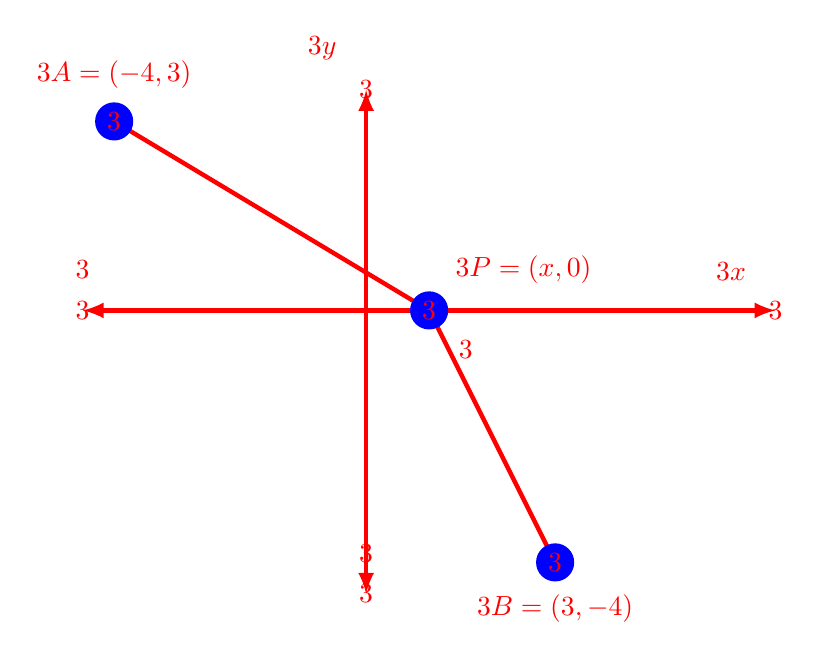
\begin{tikzpicture}[scale=0.8,
fontscale=3,
         dot/.style = {
     fill = blue,
      circle,
      inner sep =2pt,
      minimum size = 4pt
    }
  ]
%%%%%%%%%%%%%%%%%%%%%%%%%%%%%%%%%%%%%%
 %\draw [very thin, style=gray!50, step=0.5] (-3,-2) grid (3,2);
 %\draw [thin, gray!60] (0,0) grid (9,9);
\coordinate (O) at (0,0);
\coordinate (Y) at (0,3.5);
\coordinate (X) at (6.5,0);
\coordinate (X1) at (-4.5,0);
\coordinate (Y1) at (0,-4.5);
 \coordinate (A) at( -4,3);
 \coordinate (B) at (3,-4);
\coordinate (P) at (1,0);
%%%%%%%%%%%%%%ejes
\draw[color=red,ultra thick,latex-latex]           (X)node[label={above left:$x$}
                               ] {} -- (X1) node[
                               label = {above:$$}] {};
\draw[color=red,ultra thick,latex-latex]           (Y)node[,label={above left:$y$}
                               ] {} -- (Y1) node[
                               label = {above:$$}] {};
%%%%%%%%%%%%%%%%%%%%%%%%%%%%
\draw[color=red,ultra thick]           (P)node[
                               label = {below right:$$}]{}-- (B) node[dot,
                                label = {below:$B=(3,-4)$}] {};
\draw[color=red,ultra thick]           (A)node[dot,
                               label = {above:$A=(-4,3)$}]{}-- (P) node[dot,
                                label = {above right:$P=(x,0)$}] {};

%   \pic [red,draw, -latex, "$\vartheta$", angle eccentricity=1.2,angle radius=1cm] {angle =C--A--O};

   \end{tikzpicture}
